\documentclass[12pt]{article}
\usepackage[top=2cm, bottom=2cm, left=2cm, right=2cm]{geometry}
\usepackage{fancyhdr}
\usepackage{graphicx}
\usepackage{hyperref}
\usepackage[utf8]{inputenc}
\usepackage[T1]{fontenc}
\setlength{\parindent}{0pt}
%\usepackage{hyperref}  %table des matières contient des
						%liens pour aller directement au section

\begin{document}
\begin{titlepage}
\begin{center}


\includegraphics[scale=0.4]{logo.png}\\[3cm]

{\huge Cahier des charges}\\[1cm]

\rule{\linewidth}{0.5mm} \\[0.4cm]
{ \huge \bfseries Amélioration d’un programme de cartographie par séquençage: création d’une interface
d’entrée/sortie. \\[0.4cm] }
\rule{\linewidth}{0.5mm} \\[1.5cm]

\noindent
\begin{minipage}{0.4\textwidth}
  \begin{flushleft} \large
    \emph{Auteurs :}\\
    Hermes \textsc{Paraqindes}\\
    Juliette \textsc{Geoffray}\\
    Eric \textsc{Cumunel}
  \end{flushleft}
\end{minipage}%
\begin{minipage}{0.4\textwidth}
  \begin{flushright} \large
    \emph{Encadrants :} \\
    Fabrice \textsc{Besnard}\\
    Laurent \textsc{Gueguen}\\
  \end{flushright}
\end{minipage}\\[4cm]

{\large 12 Février 2018}

\end{center}
\end{titlepage}

\clearpage
\tableofcontents

\newpage

\section{Présentation du projet}
\subsection{Contexte}

La mutagenèse est un processus par lequel l'information génétique d'un organisme, et donc celle de son ADN est modifiée, ce qui entraîne une mutation.

L'apparition des mutants dans une population est un phénomène rare et donc avec une très faible probabilité de se produire. Afin d'augmenter cette probabilité, les organismes peuvent être traités par des agents mutagènes qui vont introduire des mutations (remplacement, modification ou endommagement) sur l'organisme de manière aléatoire. Ces agents mutagènes peuvent être de nature chimique comme EMS (Méthanesulfonate d'éthyle),de nature physique comme la lumière ultraviolette et les radiations ionisantes ou de nature bactérienne pathogénique contenant des plasmides (ex: T DNA) capables de d’intégrer au génome de l'hôte une séquence ADN (capable de s'exprimer ou non). 

Provoquer des mutations dans un organisme d’intérêt permet de localiser les gènes d’intérêts, de les cartographier et d'en déduire des informations sur le rôle des gènes. L'identification des mutations responsables du phénotype du mutant constitue le principe de base de la génétique mendélienne. La méthode utilisée pour identifier la mutation recherchée est celle du clonage positionnel.

C'est une méthode utilisée dans les cas où on ne connaît ni la séquence, ni la fonction du gène mais dont la mutation est supposée être à l'origine d'un caractère phénotypique visible. Un croisement avec une lignée génétiquement différente n'ayant pas le phénotype mutant est réalisé. Suite au croisement, il est nécessaire de génotyper un grand nombre d'individu et cela est une tâche fastidieuse prenant beaucoup de temps. La révolution dans les nouvelles technologies de séquençage et d'assemblage du génome a facilité le processus. Aujourd'hui on peut séquencer plusieurs mutants en même temps et analyser les variations génomiques sur tout le génome en une seule fois.

Toutefois, c'est une analyse bio-informatique qui requiert de nombreuses étapes ainsi que l'utilisation de plusieurs programmes et logiciels distincts. La plupart des programmes utilisés sont adaptés à un organisme modèle ou à un « design » génétique, et dépendent de serveurs distants. Afin de faciliter l'étape de cartographie et l'identification des mutations, un pipeline appelé \textit{Andalusian\_Mapping} a été développé. Ce pipeline permet de travailler avec différentes espèces et souches de cartographie.

\subsection{Objectifs}

L'objectif général de ce projet est de rendre \textit{Andalusian\_Mapping} plus accessible à la communauté scientifique, notamment pour les biologistes non-informaticiens, à la fois au niveau de la mise en place des outils du pipeline que de l'affichage des résultats.

Pour ce faire, plusieurs pistes peuvent se révéler intéressantes : 

\begin{itemize}
\item Au niveau de la mise en place : incorporer le programme dans un docker contenant les dépendances logicielles nécessaires
\item Au niveau de l'importation des données de départ : intégrer une interface graphique permettant d'ajouter les fichiers plus aisément
\item Au niveau de l'exploitation des résultats finaux : créer une interface graphique et/ou une page HTML pour visualiser les différents résultats (sous la forme de graphes et de tableau)
\item Améliorer l'organisation du pipeline (optionnel) 
\end{itemize}

\subsection{Description de l'existant}

Récemment, Cloudmap, un pipeline automatique de mapping-by-sequencing et d'identification de mutants a été développé et intégré à Galaxy, qui est une interface utilisateur simple et intuitive.
Cependant, ce pipeline ne permet pas à ce jour de travailler avec des génomes de référence \textit{exotiques}, étant donné que seuls les gènomes modèles comme \textit{Caenorhabditis elegans} ou \textit{Arabidopsis thaliana} sont disponibles sur Galaxy.
\textit{Andalusian Mapping} a donc été développé dans le but de fournir un outil similaire afin de travailler avec une gamme plus vaste d'organisme.

\textit{Andalusian Mapping} est un pipeline permettant d'effectuer une cartographie par séquençage afin d'identifier les régions les plus susceptibles d'être responsables d'une mutation.
Ce pipeline est un script bash permettant l'utilisation en une seule étape de plusieurs outils bioinformatiques. \\
Il tourne sous environnement Linux et Mac. La mise en place de différents logiciels est cependant fastidieuse et nécessaire au fonctionnement de ce pipeline.

Logiciels requis :

\begin{itemize}
\item bwa version 0.7.5a-r405 ou supérieur
\item samtools version 0.1.18 ou supérieur
\item Picard Version 1.110 ou supérieur
\item GATK Version 3.7 ou supérieur
\item R Version 3.3 ou supérieur, avec le package ggplot2.
\item snpEff Version 4.1g ou supérieur
\end{itemize}


L'utilisation de ce pipeline se base sur un fichier de configuration à remplir préalablement contenant les chemins vers les exécutables des logiciels utilisés, les fichiers \textit{fastq}, le génome de référence, une liste de variants prédéfinie ainsi qu'un répertoire dans lequel seront envoyés les résultats intermédiaires et finaux.\\

Description du pipeline dans son ensemble :
\begin{enumerate}

\item Mapping et sorting des lectures contre le gènome de référence avec BWA
\item Ajout des informations de groupe de lectures
\item Merge des duplicats de lecture détectés
\item Indexation du fichier BAM
\item Génération de statistiques d'alignement (fréquence, couverture)
\item Réalignement des lectures en prenant en compte les informations récoltées jusqu'ici
\item Base Quality Score Recalibration avec génération de graphique et de statistique de qualité
\item Variant Calling
\item Réalisation de la cartographie des mutations à l'aide des SNP connus pour chaque scaffold
\item Détection des meilleurs locus candidats grâce aux annotations.
\item Génération des graphiques à l'aide d'un script R et d'un fichier contenant les locus les plus probables d'être responsables de la mutation
\end{enumerate}


\item La première étape consiste à aligner les reads contre un génome de référence et à trier le fichier de sortie (.bam) pour les besoins d'un logiciel intervenant plus tard (PICARD). 
\item Ensuite on ajoute des informations de groupes aux reads.
\item L'étape suivante consiste au merge des séquence et la suppression des reads dupliqué. 
\item On indexe le fichier bam pour les besoins d'un logiciel intervenant plus tard (picard). 
\item Génération de statistiques.
\item On réaligne les reads en prenant en compte les informations récolter jusqu'ici dans le pipeline
\item On réalise une étape de Base Quality Score Recalibration avec génération de graphique et de statistique de qualité.
\item On réalise l'appel de variant. 
\item On va réaliser la cartographie de la mutation et on calcul la fréquence de l'allèle JU170 pour chaque scafold. 
\item On va trouver les meilleurs locus candidats grâce au annotation. 
\item On va générer des graphiques a l'aide de R et un fichier texte comprenant les locus responsable de la mutation les plus probables. 
\end{enumerate}

\begin{center} 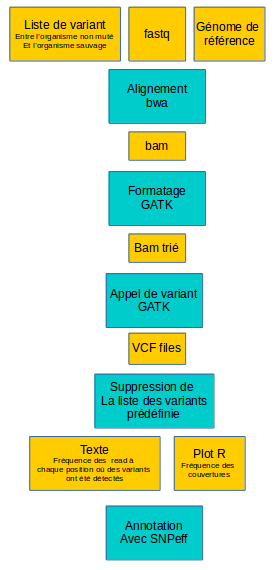
\includegraphics[scale=0.8]{schemaPipeline.png} \end{center}

\subsection{Critères d'acceptabilité du produit}

Afin de répondre à la problématique, une interface graphique sera développée. Elle devra permettre la rédaction du formulaire en entrée de pipeline, son exécution et enfin, la visualisation des résultats de sorties.

Le logiciel devra être simple d'utilisation et les résultats facilement interprétables.

\section{Expression des besoins}
\subsection{Besoins fonctionnels}

\newpage

\subsubsection{Fonctionnalité du logiciel}

Le logiciel devra remplir la même fonction que précédemment, tout en présentant une mise en place simplifiée et une visualisation des résultats améliorée, afin de permettre à des utilisateurs possédant peu de connaissances en informatique de l'utiliser.

\subsubsection{Fonctionnalité du code}

Les fonctionnalités que doit remplir le code permettant la rédaction du fichier d'entrée du pipeline:

\begin{itemize}
\item remplir les champs du fichier source (configuration du pipeline) :
\begin{itemize}
\item Génome de référence
\item Fastq en pairend 
\item Liste d'allèles connus entre l'individu sauvage et l’individu pas encore muté. Pour pouvoir les supprimer lors de l'appel de variant entre l'organisme sauvage et l'organisme muté. 
\item Données d'information sur les reads (comme la technique de séquençage utilisée ex: Illumina, le SNP utilisé pour repérer la région mutée...)
\item Le nom de sortie du dossier et de l’extension ajoutée au fichier.
\end{itemize}
\item Dans un second temps, on pourra prévoir un remplissage de certains champs automatiquement via des pipelines développés par le maître d'ouvrage. Comme la génération de la liste des variant entre l'organisme sauvage et l'organisme pas encore muté.
\end{itemize}

Les fonctionnalités que doit remplir le code permettant la sortie des résultats: 

\begin{itemize}
\item Visualisation claire des données et des graphiques d’intérêt.
\item Un fichier de sortie exportable comme une page html, pour facilité le partage de ces résultats. 
\end{itemize}

\subsection{Besoins non fonctionnels}

L'interface développée est réalisée sous le système d'exploitation Linux, il comprendra des parties en Shell, en Python et on utilisera également \textit{pyQt}, une librairie graphique python.

\section{Contraintes}
\subsection{Délais}

Le projet s'organise sur une période de 4 semaines. Il débutera le lundi 5 février et prendra fin le vendredi 2 mars. Le projet pourra être continué durant une période de cours allant du 5 au 29 mars.

Un cahier des charges définitif devra être présenté le lundi 12 février.

Le délivrable final devra être rendu le 29 mars 2018.

\subsection{Autres contraintes}
\section{Déroulement du projet}
\subsection{Planification}

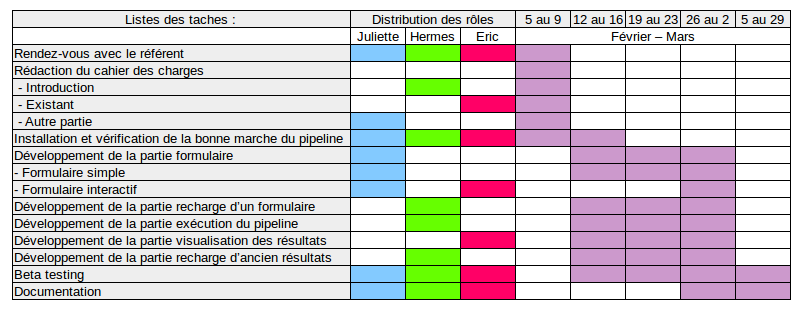
\includegraphics[scale=0.6]{gantt5.png}

\subsection{Plan d'assurance qualité}

Le contrôle qualité de l'interface développée consistera en une bonne exécution, simple et sans erreurs. Le logiciel sera testé par des membres de différentes équipes :

\begin{itemize}
\item Validation par Dr Besnard
\item Utilisation du logiciel par des utilisateurs non initiés en informatique
\end{itemize}

\subsection{Responsabilités}
\subsubsection{Maîtrise d'ouvrage}

Ce projet nous a été proposé par Fabrice Besnard, biologiste rattaché à l’École Normale Supérieur de Lyon (ENS), travaillant au Laboratoire de Reproduction et Développement des Plantes (RDP).

\subsubsection{Maîtrise d’œuvre}

Pour réaliser ce projet, nous serons trois étudiants en Master 1 de Bio-informatique à Lyon 1 : Juliette Geoffray, Hermes Paraqindes et Eric Cumunel.

\section{Bibliographie}
\begin{enumerate}
\item Schneeberger, K. Using next-generation sequencing to isolate mutant genes from forward genetic screens. Nat. Rev.
Genet. 15, 662–676 (2014).
\item Galaxy | Published Page | CloudMap. Available at: https://usegalaxy.org/u/gm2123/p/cloudmap. (Accessed: 5th
September 2017)
\item Home of SHOREmap. Available at: http://bioinfo.mpipz.mpg.de/shoremap/index.html. (Accessed: 5th September
2017)
\item MutMap - Genomics \& Breeding. Available at: http://genome-e.ibrc.or.jp/home/bioinformatics-team/mutmap.
(Accessed: 5th September 2017)
\item Besnard, F., Koutsovoulos, G., Dieudonné, S., Blaxter, M. \& Félix, M.-A. Toward Universal Forward Genetics:
Using a Draft Genome Sequence of the Nematode Oscheius tipulae To Identify Mutations Affecting Vulva
Development. Genetics 206, 1747–1761 (2017).
\item Besnard, F. Andalusian\_Mapping: Scripts to perform mapping-by-sequencing. (2017).
\end{enumerate}

\end{document}
